\documentclass[11pt]{beamer}
% Nastavení znakové sady Unicode
\usepackage{cmap}
\usetheme{Madrid}
\usepackage[utf8]{inputenc}
\usepackage[czech]{babel}
\usepackage[T1]{fontenc}
\usepackage{graphicx}
\usepackage{url}
\usepackage{hyperref}
\author[Roman Ondráček]{Roman Ondráček}
\title[Měření a regulace teploty]{Měření a regulace teploty v~domácnosti}
\setbeamercovered{transparent}
\institute[]{Gymnázium Boskovice}
\date{\today}
%\subject{}
\begin{document}

\begin{frame}
\titlepage
\end{frame}

\begin{frame}{Obsah}
\tableofcontents
\end{frame}

\section{Co bylo cílem projektu}

\begin{frame}{Co bylo cílem projektu}
  V~posledních létech je ve středu pozornosti tzv. Internet věcí a chytrá domácnost. \\[4mm]
  Cílem této práce je navrhnout a sestavit senzor teploty a zařízení, které bude teplotu regulovat.
\end{frame}

\section{Použité technologie}

\begin{frame}{Použité technologie}
  \begin{exampleblock}{Brána}
    \begin{itemize}
      \item Raspberry Pi 3; Raspbian (Debian)
      \item MQTT broker mosquitto
      \item IQRF Gateway Daemon a IQRF Gateway Daemon Webapp
      \item Node-RED
    \end{itemize}
  \end{exampleblock}
  \begin{block}{Senzor teploty a vlhkosti}
    \begin{itemize}
      \item Mikrokontrolér Atmel ATmega328P-PU
      \item Senzor teploty a vlhkosti Bosh BME280
      \item Ethernetový řadič WIZnet W5100
    \end{itemize}
  \end{block}
  \begin{alertblock}{PWM regulátor ventilátoru}
    \begin{itemize}
      \item Bezdrátový modul IQRF TR-72DAT
    \end{itemize}
  \end{alertblock}
\end{frame}

\subsection{Bezdrátový modul IQRF}

\begin{frame}{Bezdrátový modul IQRF}
  Použil jsem bezdrátový modul IQRF TR-72DAT, který vyvíjí česká firma IQRF Tech s.r.o., která sídlí v Jičíně.
  \begin{exampleblock}{Výhody}
    \begin{itemize}
      \item Malé rozměry.
      \item Dobrá technická podpora.
      \item SDK je dostupné pro mnoho platforem.
      \item Komunikace je šifrována pomocí šifry AES-128.
    \end{itemize}
  \end{exampleblock}
  \begin{alertblock}{Nevýhody}
    \begin{itemize}
      \item Vyšší cena.
    \end{itemize}
  \end{alertblock}
\end{frame}

\subsection{IQRF Gateway Daemon}

\begin{frame}{IQRF Gateway Daemon}
  Pro komunikaci s~IQRF sítí je použit IQRF Gateway Daemon, což je open source software, který obstarává komunikaci mezi IQRF sítí a MQTT brokerem. \\[4mm]
  Pro uživatelsky přívětivou konfiguraci jsem vytvořil webovou aplikaci, která je napsaná ve skriptovacím jazyce PHP.
  \begin{figure}
    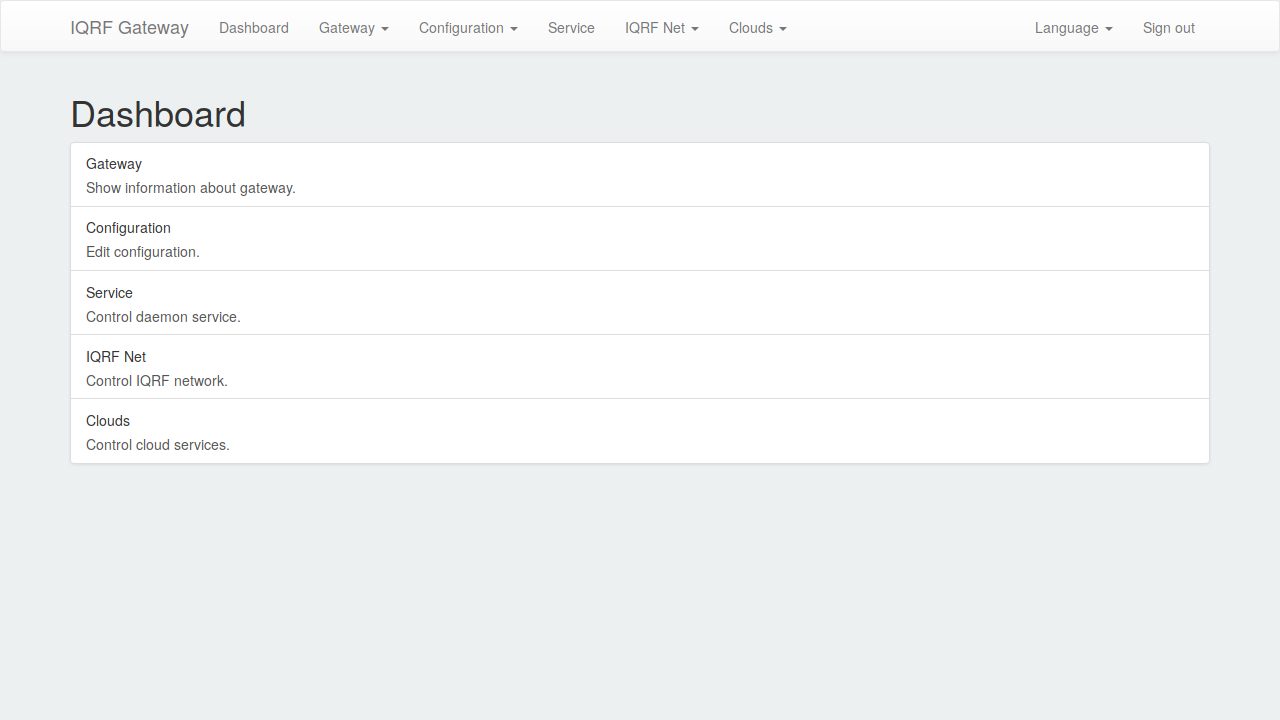
\includegraphics[width = 50mm]{../img/iqrf/iqrf-daemon-webapp.png}
    \caption{Výchozí stránka IQRF Gateway Daemon webapp}
  \end{figure}
\end{frame}

\subsection{Node-RED}

\begin{frame}{Node-RED}
  Pro zpracování a vizualizaci dat jsem zvolil nástroj Node-RED, což je open-source software původně vyvíjený společností IBM, který má za úkol usnadnění připojení zařízení do Internetu. Tento nástroj je napsán v skriptovacím jazyce JavaScript s~použitím frameworku Node.js.
  \begin{center}
    \minipage{0.50\textwidth}
      \begin{figure}
        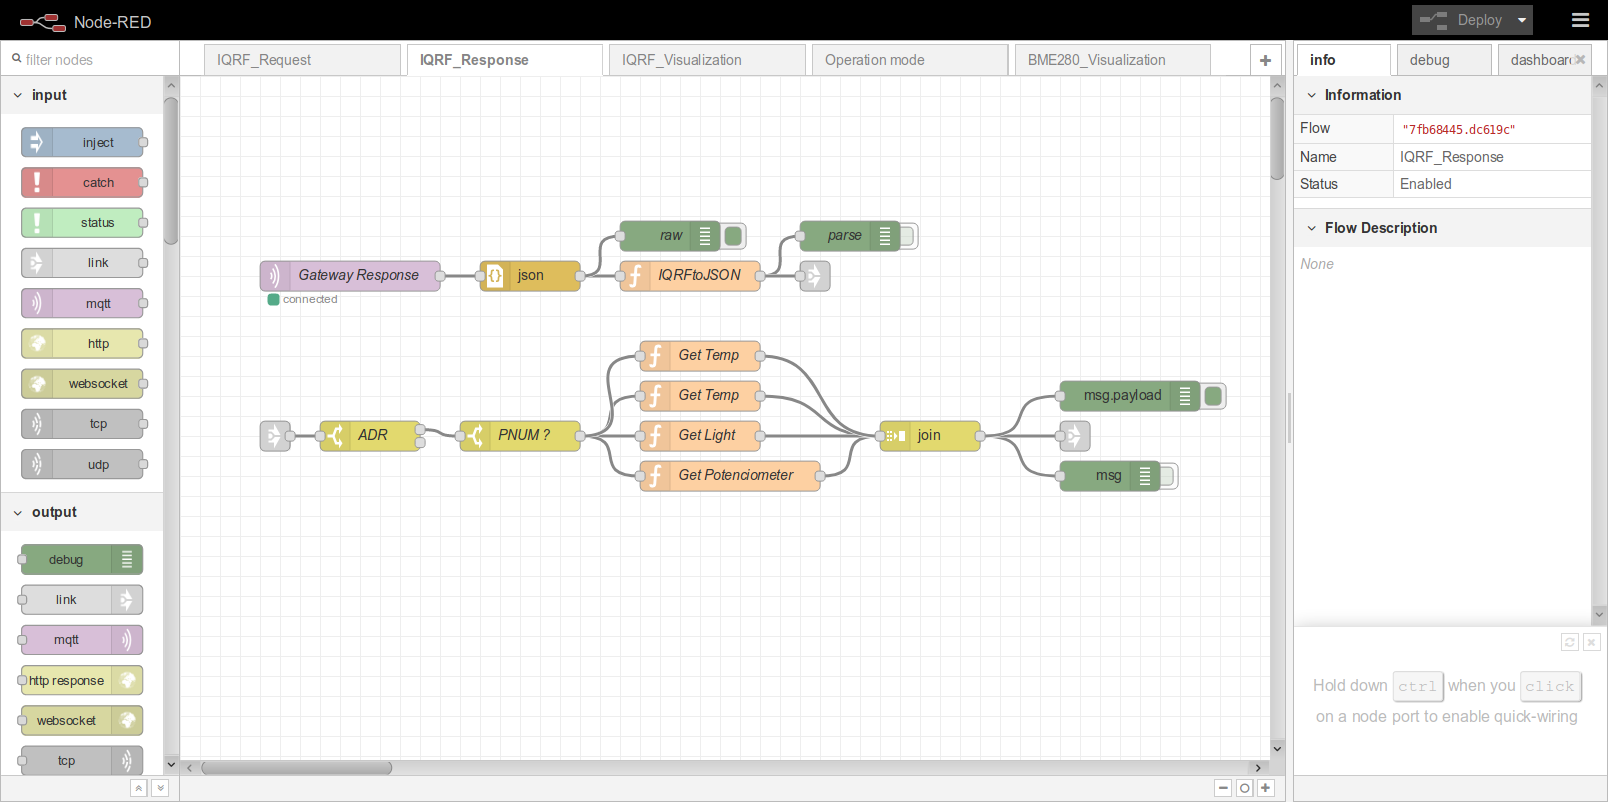
\includegraphics[width = \textwidth]{../img/node-red.png}
        \caption{Webové prostředí Node-REDu}
      \end{figure}
    \endminipage
    \minipage{0.50\textwidth}
      \begin{figure}
        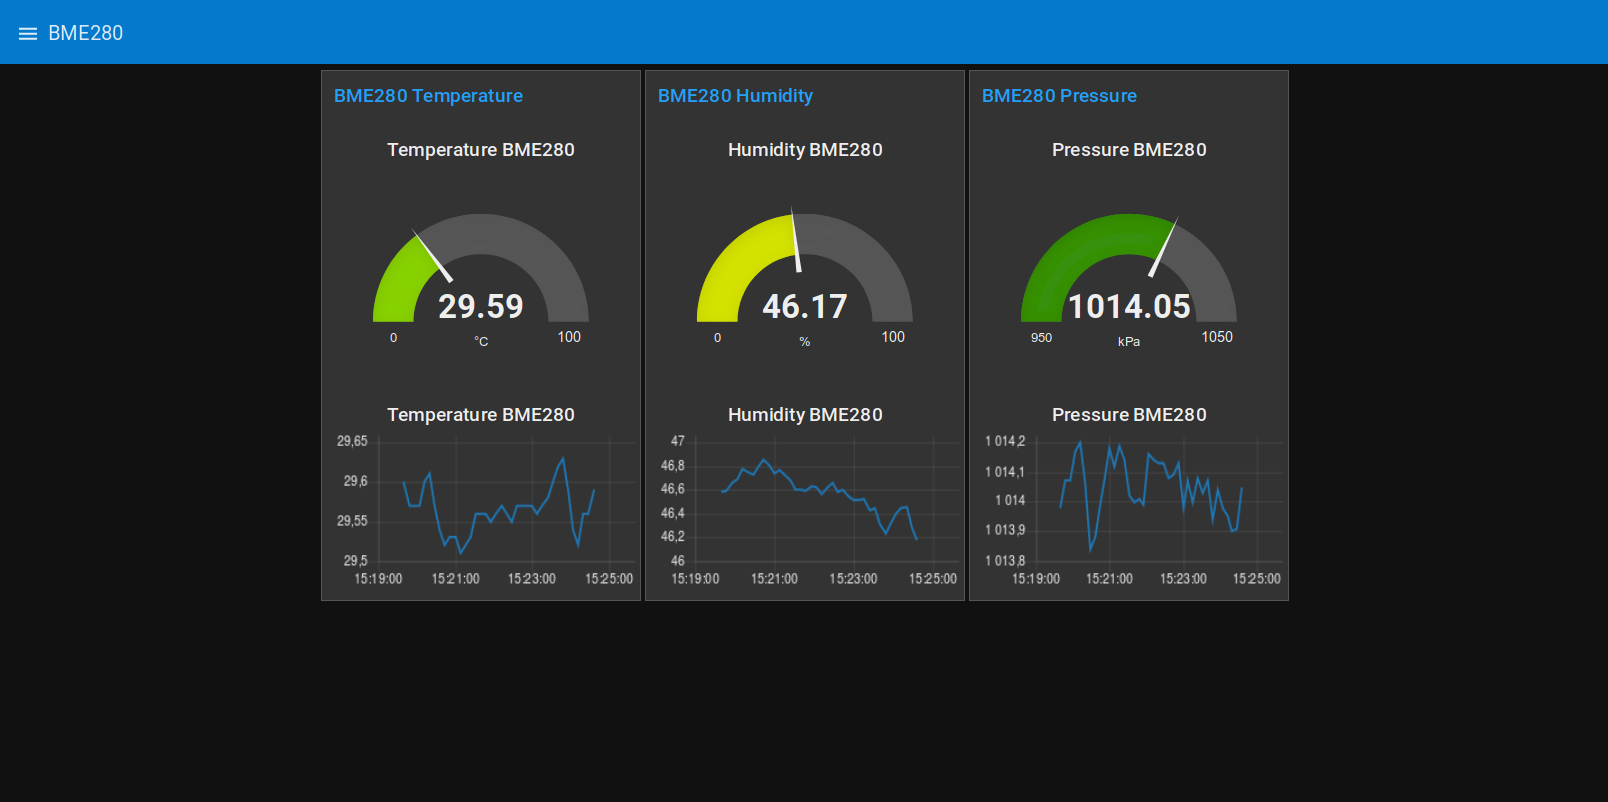
\includegraphics[width = \textwidth]{../img/node-red_dashboard.png}
        \caption{Node-RED Dashboard s grafy}
      \end{figure}
    \endminipage
  \end{center}
\end{frame}

\section{Blokové schéma komunikace}

\begin{frame}{Blokové schéma komunikace}
  \begin{center}
    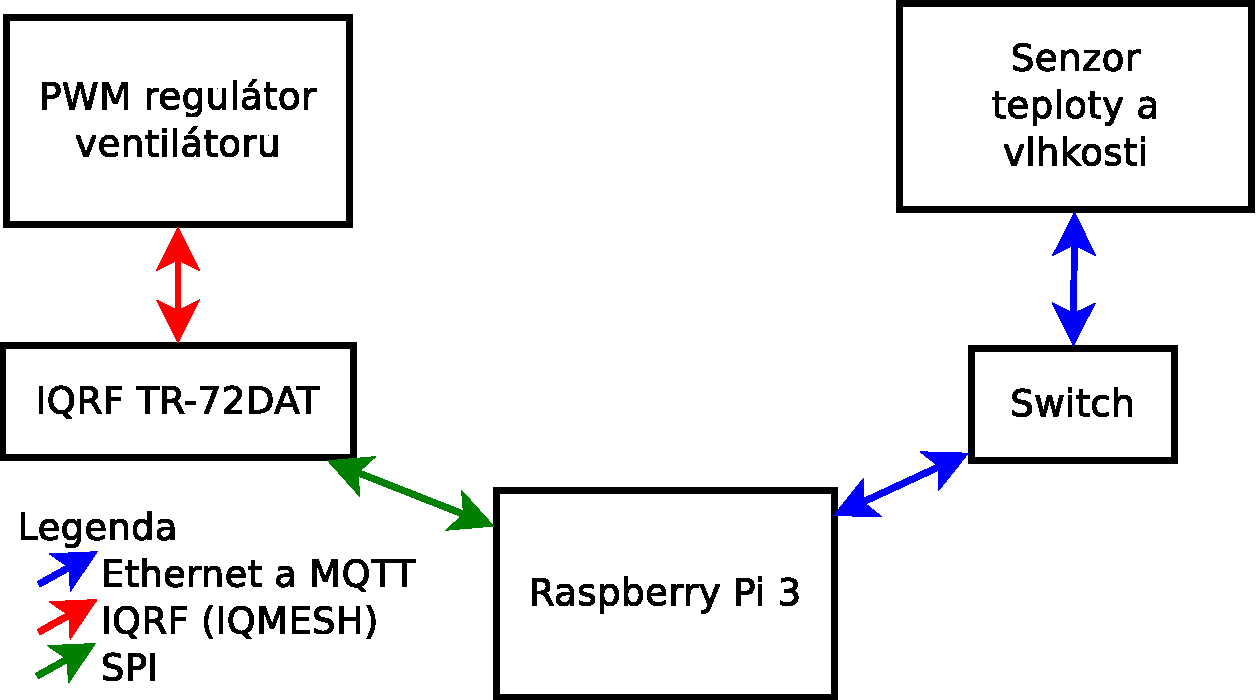
\includegraphics[width = \textwidth]{../img/blokove-schema/komunikace.pdf}
  \end{center}
\end{frame}


\section{Bloková schémata}

\begin{frame}{Bloková schémata}
  \begin{center}
    \begin{figure}
      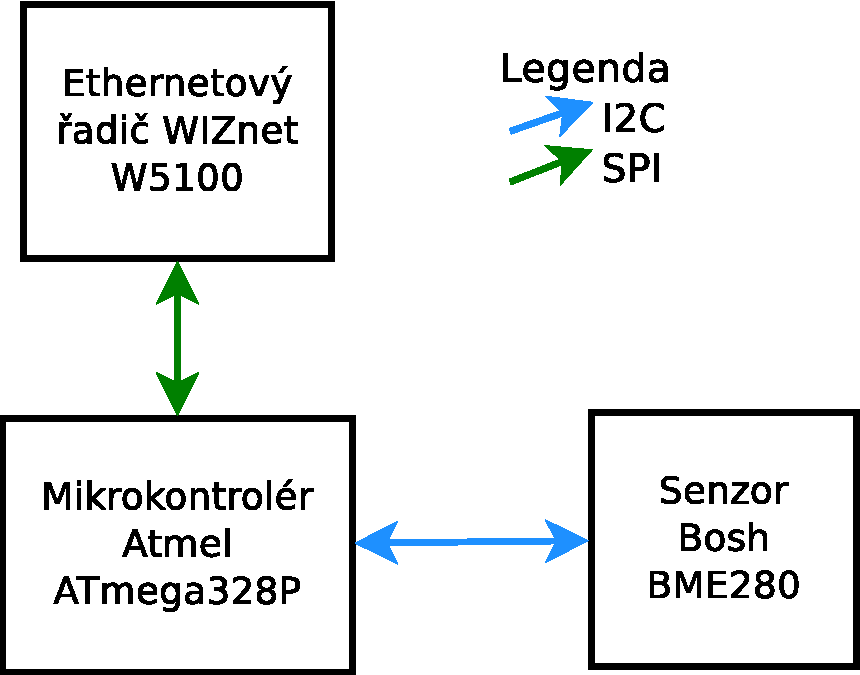
\includegraphics[width = 0.60\textwidth]{../img/blokove-schema/senzor.pdf}
      \caption{Senzor teploty a vlhkosti}
    \end{figure}
  \end{center}
\end{frame}

\section{Fotografie}

\begin{frame}{Fotografie}
  \begin{center}
    \minipage{0.50\textwidth}
      \begin{figure}
        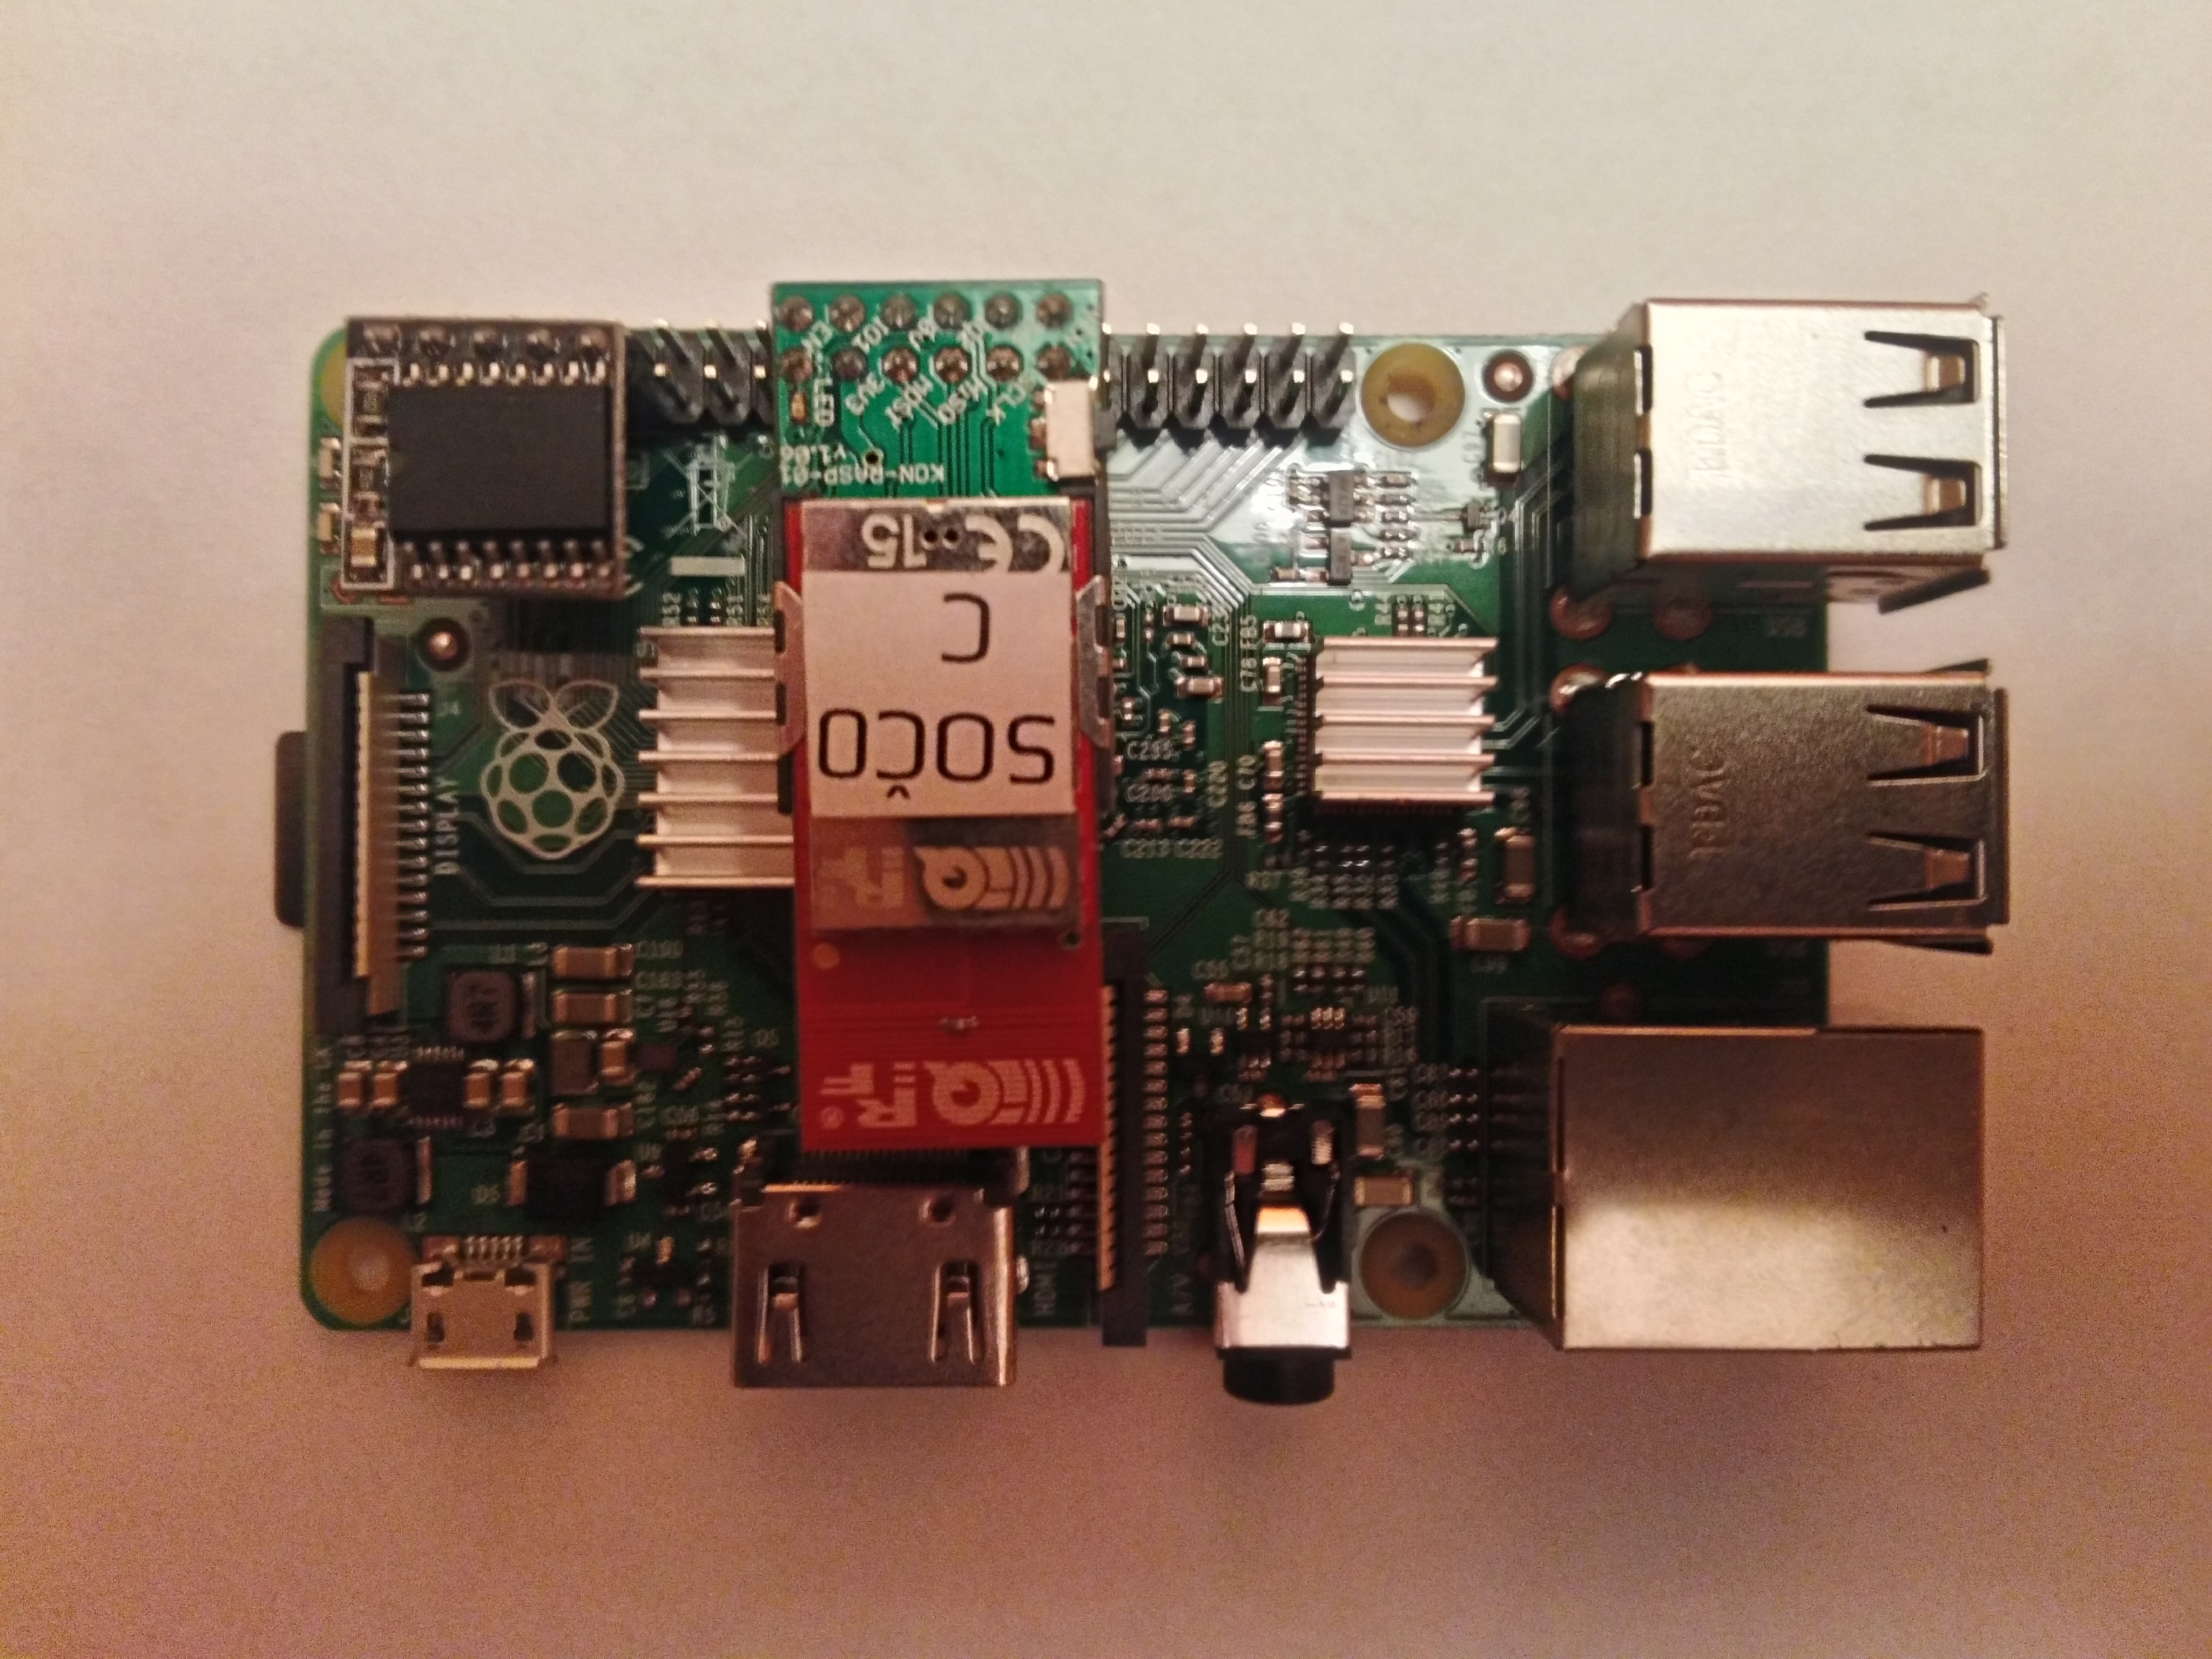
\includegraphics[width = \textwidth]{../img/foto/brana.jpg}
        \caption{Brána}
      \end{figure}
    \endminipage
    \minipage{0.50\textwidth}
      \begin{figure}
          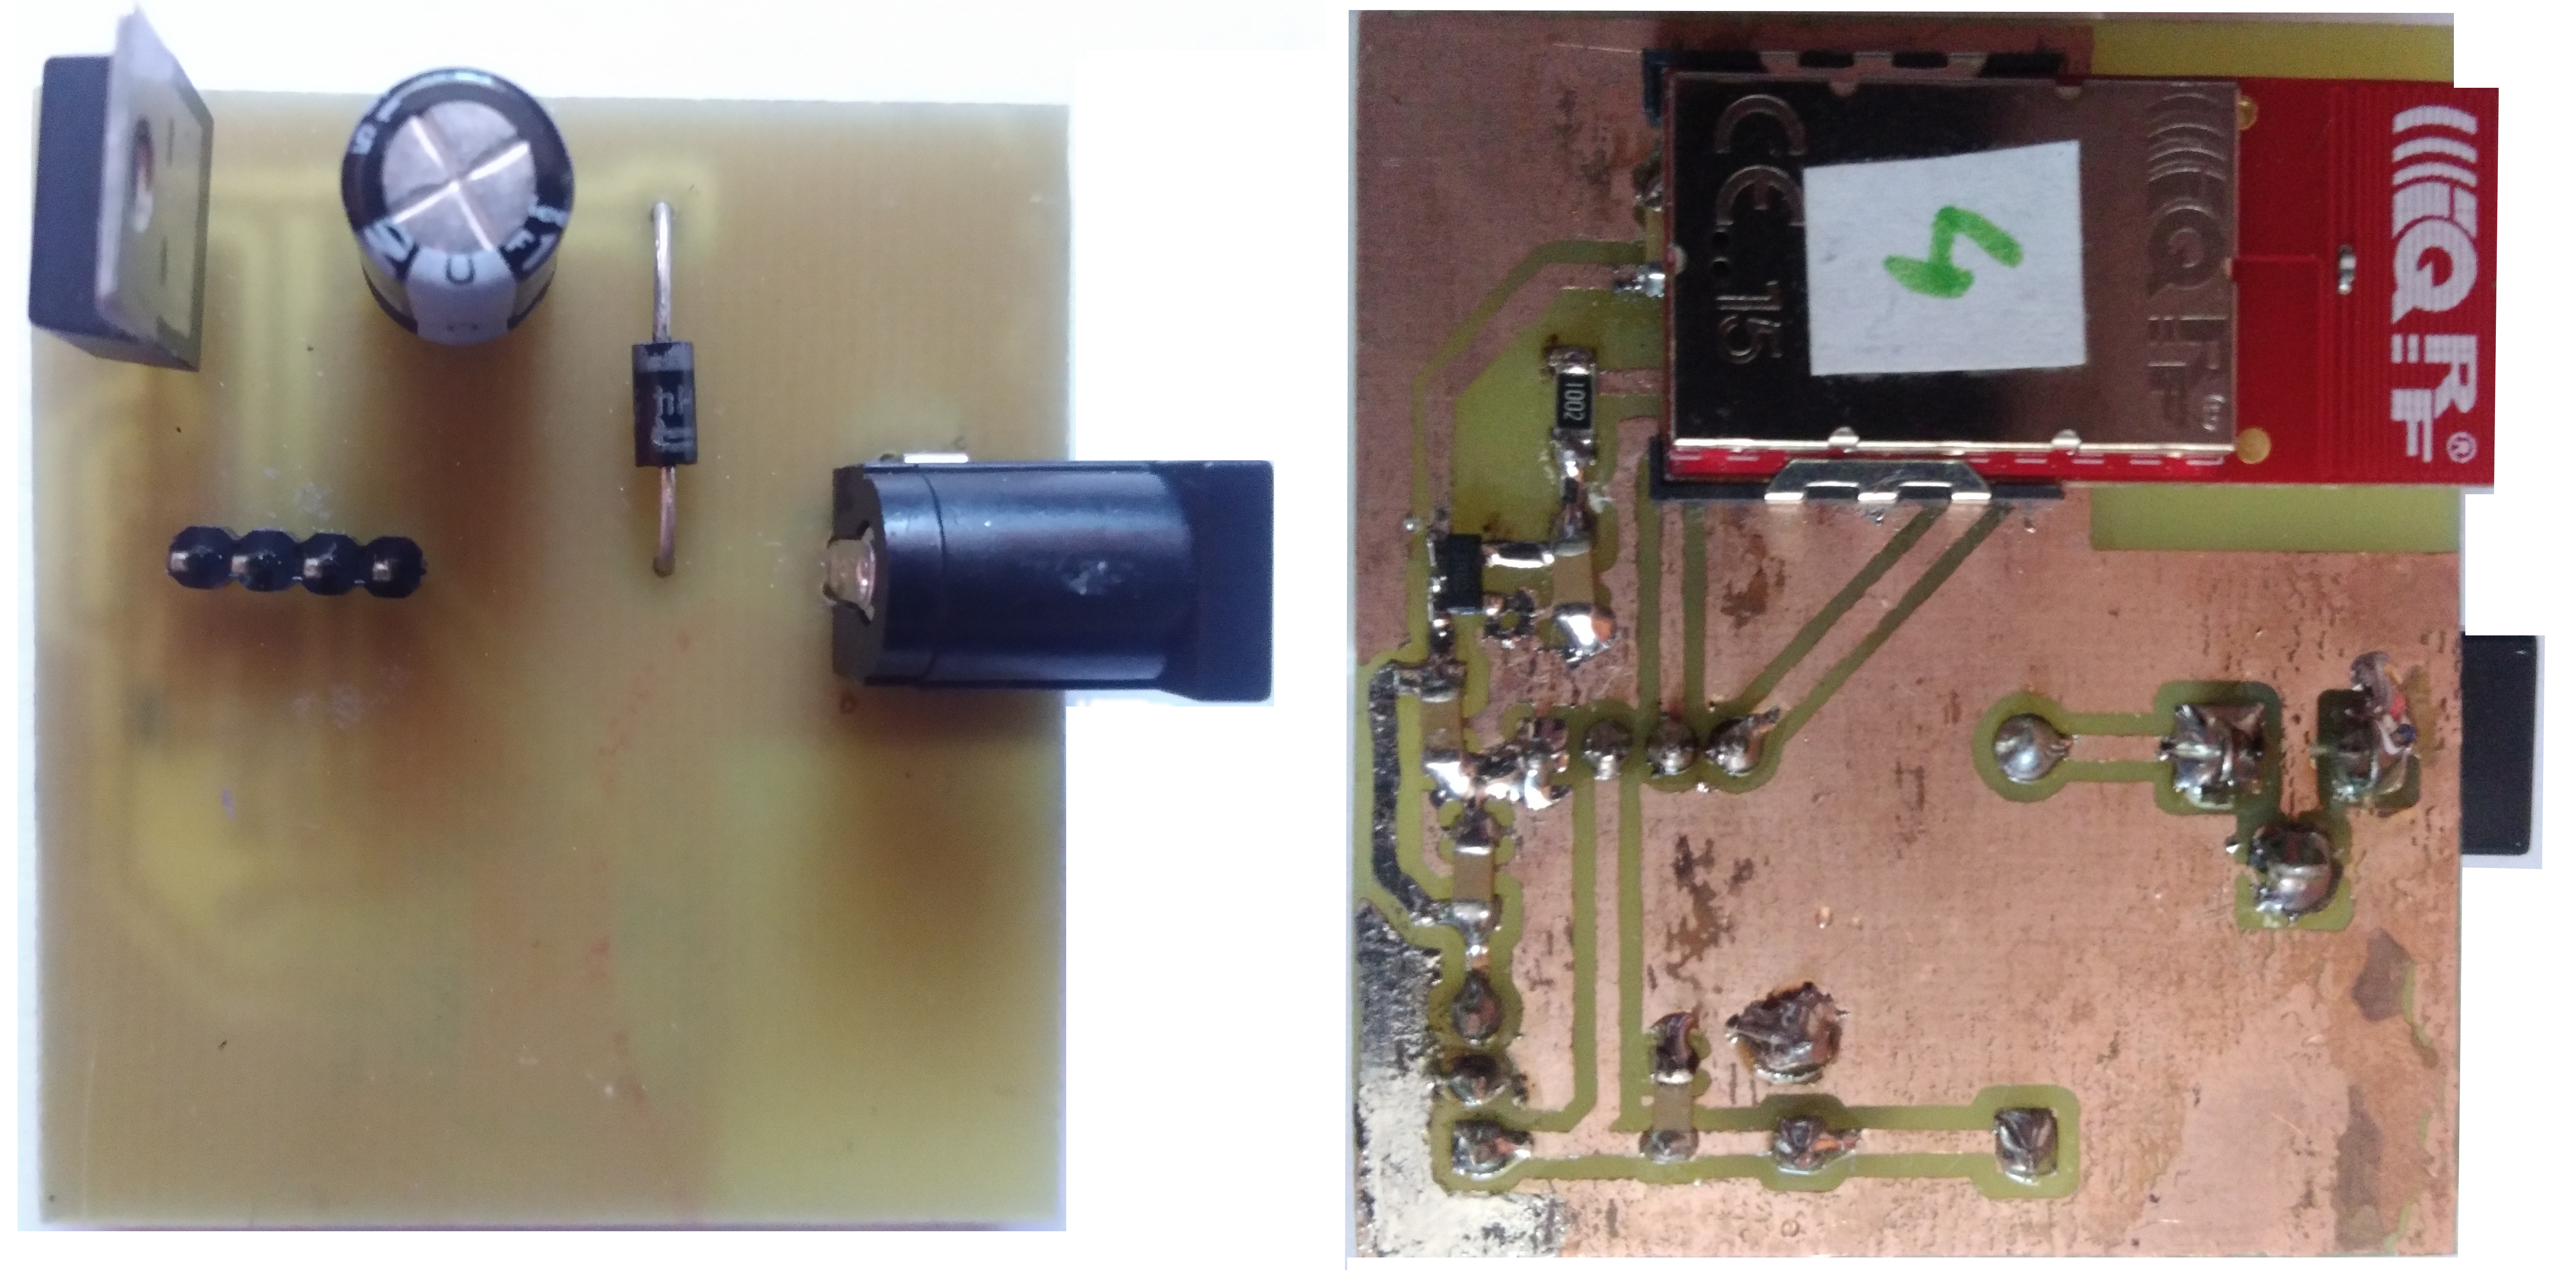
\includegraphics[width = 45mm]{../img/foto/iqrf-pwm-fan-controller.jpg}
          \caption{PWM regulátor ventilátoru}
      \end{figure}
      \begin{figure}
        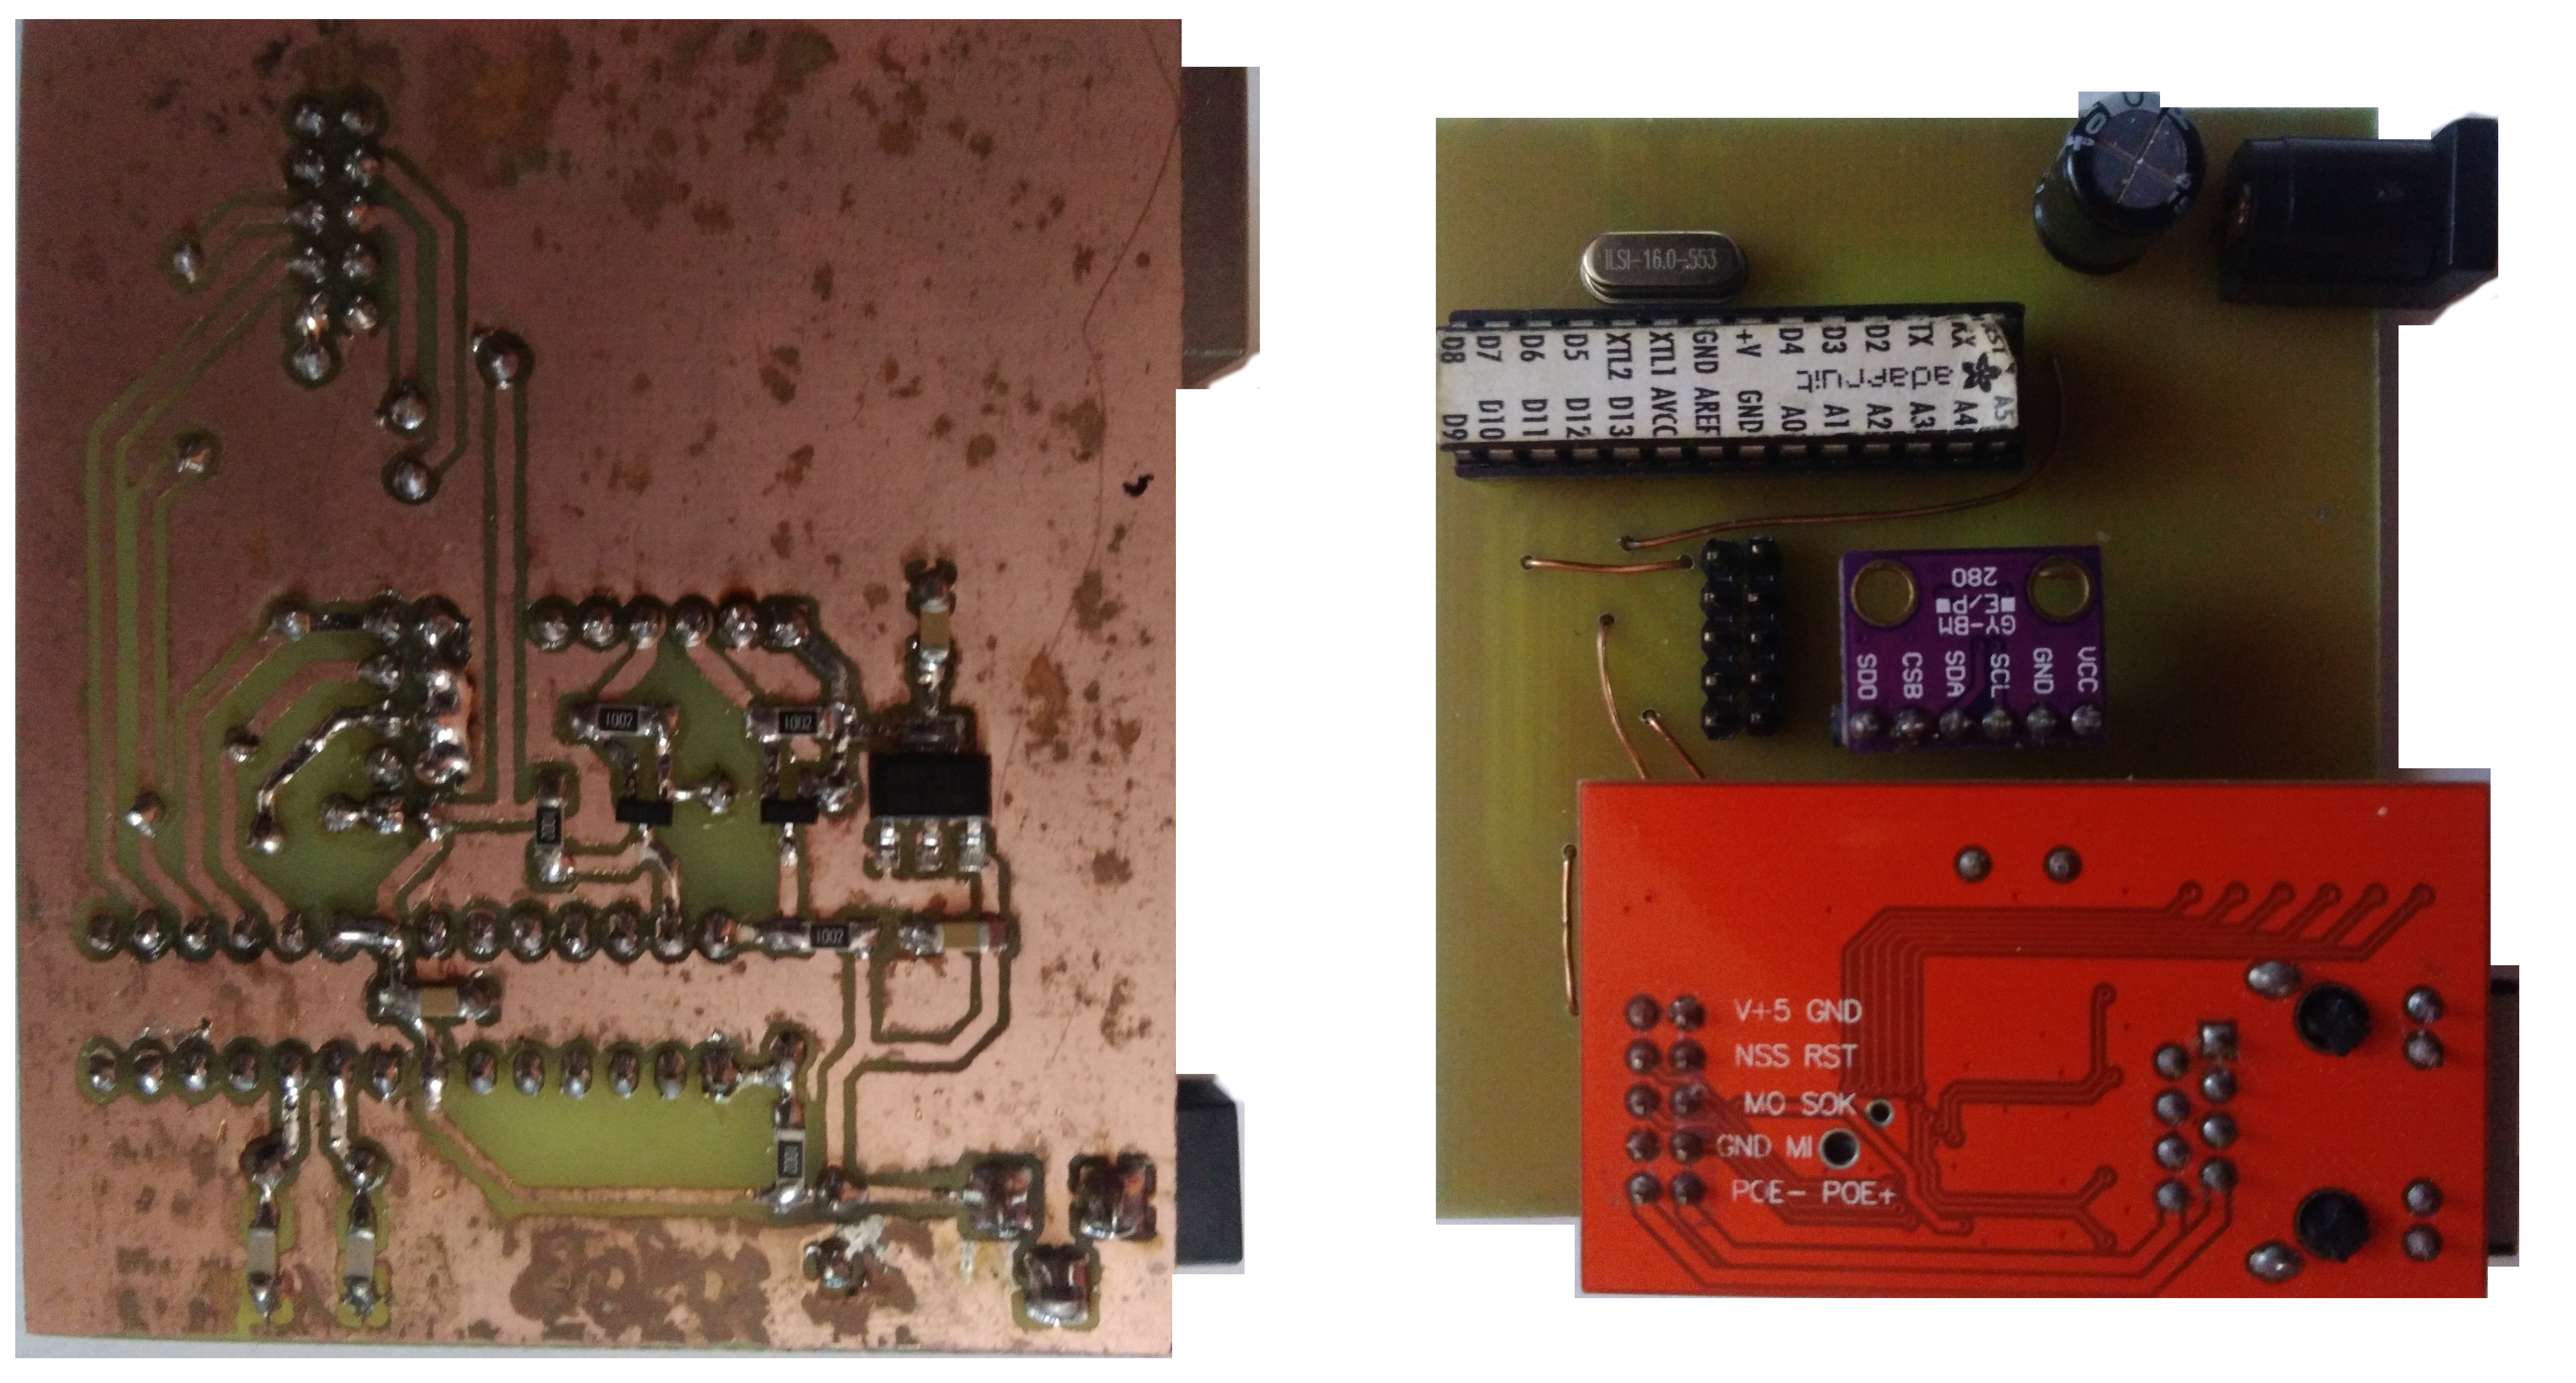
\includegraphics[width = 45mm]{../img/foto/arduino-ethernet-sensor.jpg}
        \caption{Senzor teploty a vlhkosti}
      \end{figure}
    \endminipage
  \end{center}
\end{frame}

\section{Výhody a nevýhody řešení}

\begin{frame}{Výhody a nevýhody řešení}
  \begin{exampleblock}{Výhody}
    \begin{itemize}
      \item Projekt je open-source a je vytvořen pomocí open-source nebo freeware nástrojů.
      \item Díky univerzálnosti a stavebnicovému řešení lze systém dobře rozšiřovat i o další funkce.
    \end{itemize}
  \end{exampleblock}
  \begin{alertblock}{Nevýhody}
    \begin{itemize}
      \item Vyšší cena.
    \end{itemize}
  \end{alertblock}
\end{frame}

\section{Živá ukázka}
\begin{frame}{Živá ukázka}
  \begin{center}
    \huge{\textit{Pravděpodobně} živá ukázka} \\
    \vspace{8mm}
    
\includegraphics[width = 0.33\textwidth]{../img/kocka.png}
    \vspace{8mm}
  \end{center}
  \small{Autor obrázku: Ketrina Yim (draguunthor.deviantart.com)}
\end{frame}

\section{Cíle do budoucna}

\begin{frame}{Cíle do budoucna}
  \begin{itemize}
    \item Doplnění měření otáček ventilátoru u PWM regulátoru.
    \item Nahrazení P regulátoru PI nebo PID regulátorem.
    \item Upravení softwaru chytré zásuvky, aby splňovala IQRF Standard pro binární výstup.
    \item Vytvoření LED kontroléru, který bude splňovat IQRF Standard pro světla.
  \end{itemize}
\end{frame}

\begin{frame}
  \begin{center}
    \begin{huge}
    Děkuji za pozornost. \\[8mm]
    \end{huge}
    \large{Dotazy?}\\[16mm]
    \textbf{Zdrojové kódy:} \\
    \url{https://github.com/Roman3349/maturitni-prace} \\[16mm]
  \end{center}
  Zdroje obrázků:
  \begin{itemize}
    \item[] \hspace{-8mm} \tiny{\textbf{Schrödingerova kočka:} \url{http://draguunthor.deviantart.com/art/Schrodinger-s-Cat-163302750}}
  \end{itemize}
\end{frame}

\end{document}
